\documentclass{beamer}
\setbeamercovered{transparent}
\mode<presentation>
{
  \usetheme{default}      % or try Darmstadt, Madrid, Warsaw, ...
  \usecolortheme{default} % or try albatross, beaver, crane, ...
  \usefonttheme{default}  % or try serif, structurebold, ...
  \setbeamertemplate{navigation symbols}{}
  \setbeamertemplate{caption}[numbered]
} 
\definecolor{links}{HTML}{2A1B81}
\hypersetup{colorlinks,linkcolor=,urlcolor=links}
\usepackage{tikz}
\usetikzlibrary{decorations.pathreplacing}
\usetikzlibrary{decorations.pathmorphing}
\usetikzlibrary{arrows}
\usetikzlibrary{decorations.markings}
\usetikzlibrary{decorations.pathreplacing}
\usetikzlibrary{backgrounds}
\usetikzlibrary{calc}
\usetikzlibrary{intersections}
\usetikzlibrary{decorations}
\usetikzlibrary{shapes, positioning} 
\usetikzlibrary{shadows}
\usepackage{relsize}
\tikzset{fontscale/.style = {font=\relsize{#1}}
}
\tikzstyle{line}=[draw,thick,-latex]
\setbeamerfont{block title}{size=\large}
\setbeamerfont{frametitle}{size=\Huge}

\setbeamertemplate{frametitle}[default][center]
\setbeamertemplate{footline}[frame number]
\usepackage[many]{tcolorbox}
\usepackage{empheq}

%\usepackage{3dplot} 

%\tcbset{}

%\newtcbox{\mybox}{}


\tcbset{highlight math style={colframe=red!60!black,colback=yellow!50!white,arc=4pt,boxrule=1pt,
  }}

\newtcbox{\mybox}{math upper,tcbox raise base,
  enhanced,frame hidden,boxrule=0pt,interior style={top color=green!10!white,
  bottom color=green!10!white,middle color=green!50!yellow},
  fuzzy halo=1pt with green,drop large lifted shadow}

%
% Choose how your presentation looks.
%
% For more themes, color themes and font themes, see:
% http://deic.uab.es/~iblanes/beamer_gallery/index_by_theme.html
%
\mode<presentation>
{
  \usetheme{default}      % or try Darmstadt, Madrid, Warsaw, ...
  \usecolortheme{default} % or try albatross, beaver, crane, ...
  \usefonttheme{default}  % or try serif, structurebold, ...
  \setbeamertemplate{navigation symbols}{}
  \setbeamertemplate{caption}[numbered]
} 

\usepackage[english]{babel}
\usepackage[utf8x]{inputenc}



\newcommand\pgfmathsinandcos[3]{%
  \pgfmathsetmacro#1{sin(#3)}%
  \pgfmathsetmacro#2{cos(#3)}%
}
\newcommand\LongitudePlane[3][current plane]{%
  \pgfmathsinandcos\sinEl\cosEl{#2} % elevation
  \pgfmathsinandcos\sint\cost{#3} % azimuth
  \tikzset{#1/.style={cm={\cost,\sint*\sinEl,0,\cosEl,(0,0)}}}
}

\newcommand\LatitudePlane[3][current plane]{%
  \pgfmathsinandcos\sinEl\cosEl{#2} % elevation
  \pgfmathsinandcos\sint\cost{#3} % latitude
  \pgfmathsetmacro\yshift{\cosEl*\sint}
  \tikzset{#1/.style={cm={\cost,0,0,\cost*\sinEl,(0,\yshift)}}} %
}
\newcommand\NewLatitudePlane[4][current plane]{%
  \pgfmathsinandcos\sinEl\cosEl{#3} % elevation
  \pgfmathsinandcos\sint\cost{#4} % latitude
  \pgfmathsetmacro\yshift{#2*\cosEl*\sint}
  \tikzset{#1/.style={cm={\cost,0,0,\cost*\sinEl,(0,\yshift)}}} %
}
\newcommand\DrawLongitudeCircle[2][1]{
  \LongitudePlane{\angEl}{#2}
  \tikzset{current plane/.prefix style={scale=#1}}
   % angle of "visibility"
  \pgfmathsetmacro\angVis{atan(sin(#2)*cos(\angEl)/sin(\angEl))} %
  \draw[current plane] (\angVis:1) arc (\angVis:\angVis+180:1);
  %\draw[current plane,dashed] (\angVis-180:1) arc (\angVis-180:\angVis:1);
}
\newcommand\DrawLatitudeCircle[2][1]{
  \LatitudePlane{\angEl}{#2}
  \tikzset{current plane/.prefix style={scale=#1}}
  \pgfmathsetmacro\sinVis{sin(#2)/cos(#2)*sin(\angEl)/cos(\angEl)}
  % angle of "visibility"
  \pgfmathsetmacro\angVis{asin(min(1,max(\sinVis,-1)))}
  \draw[current plane] (\angVis:1) arc (\angVis:-\angVis-180:1);
  \draw[current plane,dashed] (180-\angVis:1) arc (180-\angVis:\angVis:1);
}


\tikzset{
    MyPerspective/.style={scale=1.8,x={(-1cm,0cm)},y={(1cm,0cm)},
    z={(0cm,1.2cm)}}
        }

\title[]{Einsteins theory of relativity}
\author{Helga Holmestad}
\institute{University of Oslo}
\date{26/10-2018}


\AtBeginSection[]{
  \begin{frame}
  \vfill
  \centering
  \begin{beamercolorbox}[sep=13pt,center,shadow=true,rounded=true]{title}
    \usebeamerfont{frametitle}\insertsectionhead\par%
  \end{beamercolorbox}
  \vfill
  \end{frame}
}





\begin{document}

\begin{frame}
  \titlepage
\end{frame}

% Uncomment these lines for an automatically generated outline.
%\begin{frame}{Outline}
%  \tableofcontents
%\end{frame}

  \tikzstyle{line} = [draw, ultra thick,-latex]
      \tikzstyle{light} = [draw,ultra thick,yellow,-latex]
      \tikzstyle{lineP} = [draw, ultra thick]
      \tikzstyle{block} = [rectangle, draw, fill=blue, 
        text width=6.0cm, text centered, rounded corners, minimum height=1em]
      
\begin{frame}{\centering Special relativity}
  \begin{columns}
    \begin{column}{0.5\textwidth}
      \begin{itemize}
      \item<1->{The ether and Maxwells equations}
      \item<2->{Two postulates }
        \begin{itemize}
        \item<2->{Laws of physics are the same in all inertial reference frames}
        \item<2->{Speed of light is constant}
        \end{itemize}
      \end{itemize}
    \end{column}
    \begin{column}{0.5\textwidth}
      \begin{itemize}
        \item<3->{Ground-breaking new ideas}
        \begin{itemize}
        \item<3->{Space and time is not independent (spacetime)}
        \item<3->{Simulationous depends upon reference frames}
        %\item<7->{Synchronize if:$t_b-t_a=t_c-t_b$}
        \end{itemize}
        \end{itemize}
         \end{column}
  \end{columns}  
  \begin{center}
    \begin{tikzpicture}
        %\visible<4,5,6,7>{\node at (-2,0)(man1) {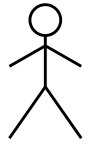
\includegraphics[width=1cm]{fig/streken.png}};  
        %\node at (2,0)(man2) {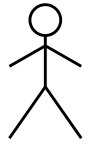
\includegraphics[width=1cm]{fig/streken.png}};  
        %\node at (-2,1){A};  
        %\node at (2,1){B};
        %}
        %\visible<5>{\path[light] ($(man1)+(4.5mm,1mm)$)--($(man2)+(-4.5mm,1mm)$);}
        %\visible<5,6,7>{
        %\node at (-2,-1.0){$t_a$};  
        %\node at (2,-1.0){$t_b$};
      %}
       % \visible<6>{\path[light] ($(man2)+(-4.5mm,1mm)$)--($(man1)+(4.5mm,1mm)$);}
        %\visible<6,7>{\node at (-2,-1.4){$t_c$};  
        %}
        
            \visible<4,5>{
              \def\x{3}
              \def\h{0}
              \def\xn{-2}
              \def\hn{-2}
              
              \node at (0.5,-1.2) {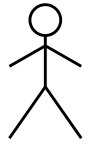
\includegraphics[width=1cm]{fig/streken.png}};
              \draw[ultra thick] (-1,-2.0) circle (0.3cm);
              \draw[ultra thick] (2,-2.0) circle (0.3cm);
              \filldraw[lineP, fill=white, draw=black] (\hn,\xn)--(\xn,\h)--(\xn,\h)--(\x,\h)--(\x,\h)--(\x,\hn)-- (\xn,\hn)--(\x,\hn);
              \node at (0.5,-1.2)(midtrain) {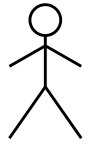
\includegraphics[width=1cm]{fig/streken.png}};
            }
            \visible<5,6>{\path[light] ($(midtrain)+(3mm,1mm)$)--($(midtrain)+(25.5mm,1mm)$);}
            \visible<5,6>{\path[light] ($(midtrain)+(-3mm,1mm)$)--($(midtrain)-(25.5mm,-1mm)$);}
           
            \visible<6->{
              \def\x{4}
              \def\h{0}
              \def\xn{-1}
              \def\hn{-2}
%          
              \draw[ultra thick] (0,-2.0) circle (0.3cm);
              \draw[ultra thick] (3,-2.0) circle (0.3cm);
              \filldraw[lineP, fill=white, draw=black] (\xn,\hn)--(\xn,\h)--(\xn,\h)--(\x,\h)--(\x,\h)--(\x,\hn)-- (\xn,\hn)--(\x,\hn);
              \node at (1.5,-1.2)(midt2) {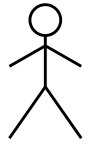
\includegraphics[width=1cm]{fig/streken.png}};
              \node at (0.5,-1.2)(midt2) {
\includegraphics[width=1cm]{fig/strekengraa.png}};
              \path[light] ($(midtrain)+(3mm,1mm)$)--($(midtrain)+(25.5mm,1mm)$);
              \path[light] ($(midtrain)+(-3mm,1mm)$)--($(midtrain)-(25.5mm,-1mm)$);
            }

        \end{tikzpicture}
      \end{center}
 \end{frame}



\begin{frame}{\centering Lorentz transformation}
 % \begin{columns}
 %   \begin{column}{0.5\textwidth}
      The transformations between two inertial reference frames moving with a velocity $v$ relative to eachoter is given by the Lorentz transformations. At t'=t=0 the origins of the two cordinates systems are the same.  
      \begin{empheq}[box=\tcbhighmath]{align*}
        t'&=\gamma(t-vx/c²)\\
        x'&=\gamma(x-vt)\\
        y'&=y\\
        z'&=z\\
        \text{where}&:\\
        c&=\text{Speed of light}\\
        \gamma&=\frac{1}{\sqrt{(1-v²/c²)}}\\
      \end{empheq}
  %    \end{column}
  \end{frame}


\begin{frame}{\centering Consequences of special relativity}
   %\node at (5,5){$\begin{aligned}v&=0.99c\\x_1&=vt\\t'&=?\\\beta&=50\end{aligned}$};
  \begin{columns}
    \begin{column}{0.2\textwidth}
      \tiny


      \begin{empheq}[box=\tcbhighmath]{align*}
    v&=0.87c\\
    \gamma&=2\\
    x_1&=\text{Back of the carpet}\\
    x_2&=\text{Front of the carpet}\\
    \visible<7->{ t_1&=\text{Start of flight}\\
    t_2&=\text{End of flight}\\}
      \end{empheq}
    \end{column}
    \begin{column}{0.35\textwidth}
      \tiny
      \only<4->{\begin{empheq}[box=\tcbhighmath]{align*}
          x'_2-x'_1&=\gamma(x_2-vt_2)-\gamma(x_1-vt_1)\\
          t_1&=t_2\\
          \Delta x'&=\gamma\Delta x\\
          \Delta x &=\frac{\Delta x'}{\gamma}
        \end{empheq}
      }
    \end{column}
    \begin{column}{0.35\textwidth}
      \tiny
      \only<8,9>{
      \begin{empheq}[box=\tcbhighmath]{align*}
        t'_2-t'_1&=\gamma(t_2-v\frac{x_2}{c^2})-\gamma(t_1-v\frac{x_1}{c^2})\\
        x_1&=vt_1,~~~x_2=vt_2\\
        t'_2-t'_1&=\gamma t_2(1-\frac{v^2}{c^2})-\gamma t_1(1-\frac{v^2}{c^2})\\
        \Delta t'&=\frac{1}{\gamma}\Delta t
      \end{empheq}
      }
    \end{column}
  \end{columns}
  %\begin{center}
    \begin{tikzpicture}
      \visible<1,2,3,4,6,7,8,9>{\node at (0,3.5){
\includegraphics[width=2.5cm,height=2.0cm]{fig/magic.png}};
      }
      \visible<2,3,4->{\draw [->, black,ultra thick] (-1,4.7) -- node[above,xshift=0cm]{\textbf{0.87c}} (1,4.7);}

      %\visible<2>{\draw [->, black,ultra thick] (-1,4.7) -- node[above,xshift=0cm]{\textbf{0.87c}} (1,4.7);}
      \linespread{0.1}
     \node[rectangle,draw,text centered, rounded corners,text width=2.0cm,fill=white] at (-5.5,2.5){\tiny{Flying on the magic carpet is the primed reference frame}};
      
     \visible<5>{\node at (0,1.5){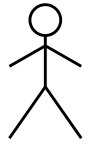
\includegraphics[width=1.0cm]{fig/streken.png}};
   }
     \visible<5>{\node at (0,3.5){
\includegraphics[width=1.5cm,height=2.0cm]{fig/magic.png}};}
     
     \visible<6,7,8,9>{\node at (0,3.65){
\includegraphics[width=0.3cm]{fig/strekenOnCarpet.png}};}
     \visible<9>{\node[rectangle,draw,text centered, rounded corners,text width=2.0cm,fill=violet!50] at (2.5,3.5){\tiny{My two hour ride was only one hour(:}};
     }
  \end{tikzpicture}
  %\end{center}


  
 
  %% \begin{tikzpicture}
  %%   \draw [->, black,very thick] (0,0) -- node[below,xshift=-0.3cm]{\textbf z} (0,5);
  %%   \draw [->, black,very thick] (0,0) --node[left,yshift=-0.3cm]{\textbf x} (5,0);
  %%   \draw [->, gray,very thick] (0,0) --node[above]{\textbf y} (1.0,1.5);
  %%   \node at (0,2.5){
\includegraphics[width=2cm]{fig/magic.png}};
  %%   \draw [->, blue,very thick] (0,0) -- node[below,xshift=-0.3cm]{\textbf z'} (0,5);
  %%   \draw [->, blue,very thick] (0,0) --node[left,yshift=-0.3cm]{\textbf x'} (5,0);
  %%   \draw [->, blue!40,very thick] (0,0) --node[above]{\textbf y'} (1.0,1.5);

  %%   \draw [->, blue,very thick] (0,0) -- node[below,xshift=-0.3cm]{\textbf z'} (0,5);
  %%   \draw [->, blue,very thick] (0,0) --node[left,yshift=-0.3cm]{\textbf x'} (5,0);
  %%   \draw [->, blue!40,very thick] (0,0) --node[above]{\textbf y'} (1.0,1.5);
    
  %%   \visible<2>{\node at (5,3){$\begin{aligned}t'_1&=\frac{t_1}{\beta}\\t_1&=\beta t'_1 \end{aligned}$};}
  %%   %\visible<2>{\node at (5,3){$\begin{aligned}t'_1&=\frac{t_1}{\beta}\\t_1&=\beta t'_1 \end{aligned}$};}    
  %%   \node at (5,2){The length of the carpet is 2~m, what is the length as seen by us};
  %%   \path[lineP] (3,-0.2)--(3,0.2) node[below,yshift=-0.5cm]{$x=x_1$};
  %%   %\visible<3>{\node at (0,0) {What is the difference between the front and the back of the magic carpent as seen from us.};}    
  %%   %\visible<4>{\node at (5,3){$\begin{aligned} x(x'=1)-x(x'=-2)=2/\beta \end{aligned}$};}
  %%   %\visible<5>{\node at (5,3){In other words we see that carpet as only 4~cm, instad of 2~m};}
      
    
  %%   %\node at (0,0){
\includegraphics[width=2cm]{fig/magic.png}};
  %% \end{tikzpicture}
\end{frame}

\begin{frame}{In the real world}
  \begin{columns}[t]
    \begin{column}{0.5\textwidth}

      ~\vspace{1.5cm}
      \begin{itemize}
      \item<1->{Atomic clocks in flights} 
      \item<2->{Muons actually reach the earth}
      \item<3->{Particle accelerators}
      \end{itemize}
      ~\vspace{5cm}
      
    \end{column}
    \begin{column}{0.6\textwidth}
      ~\vspace{1cm}\\
      
      \only<1>{
        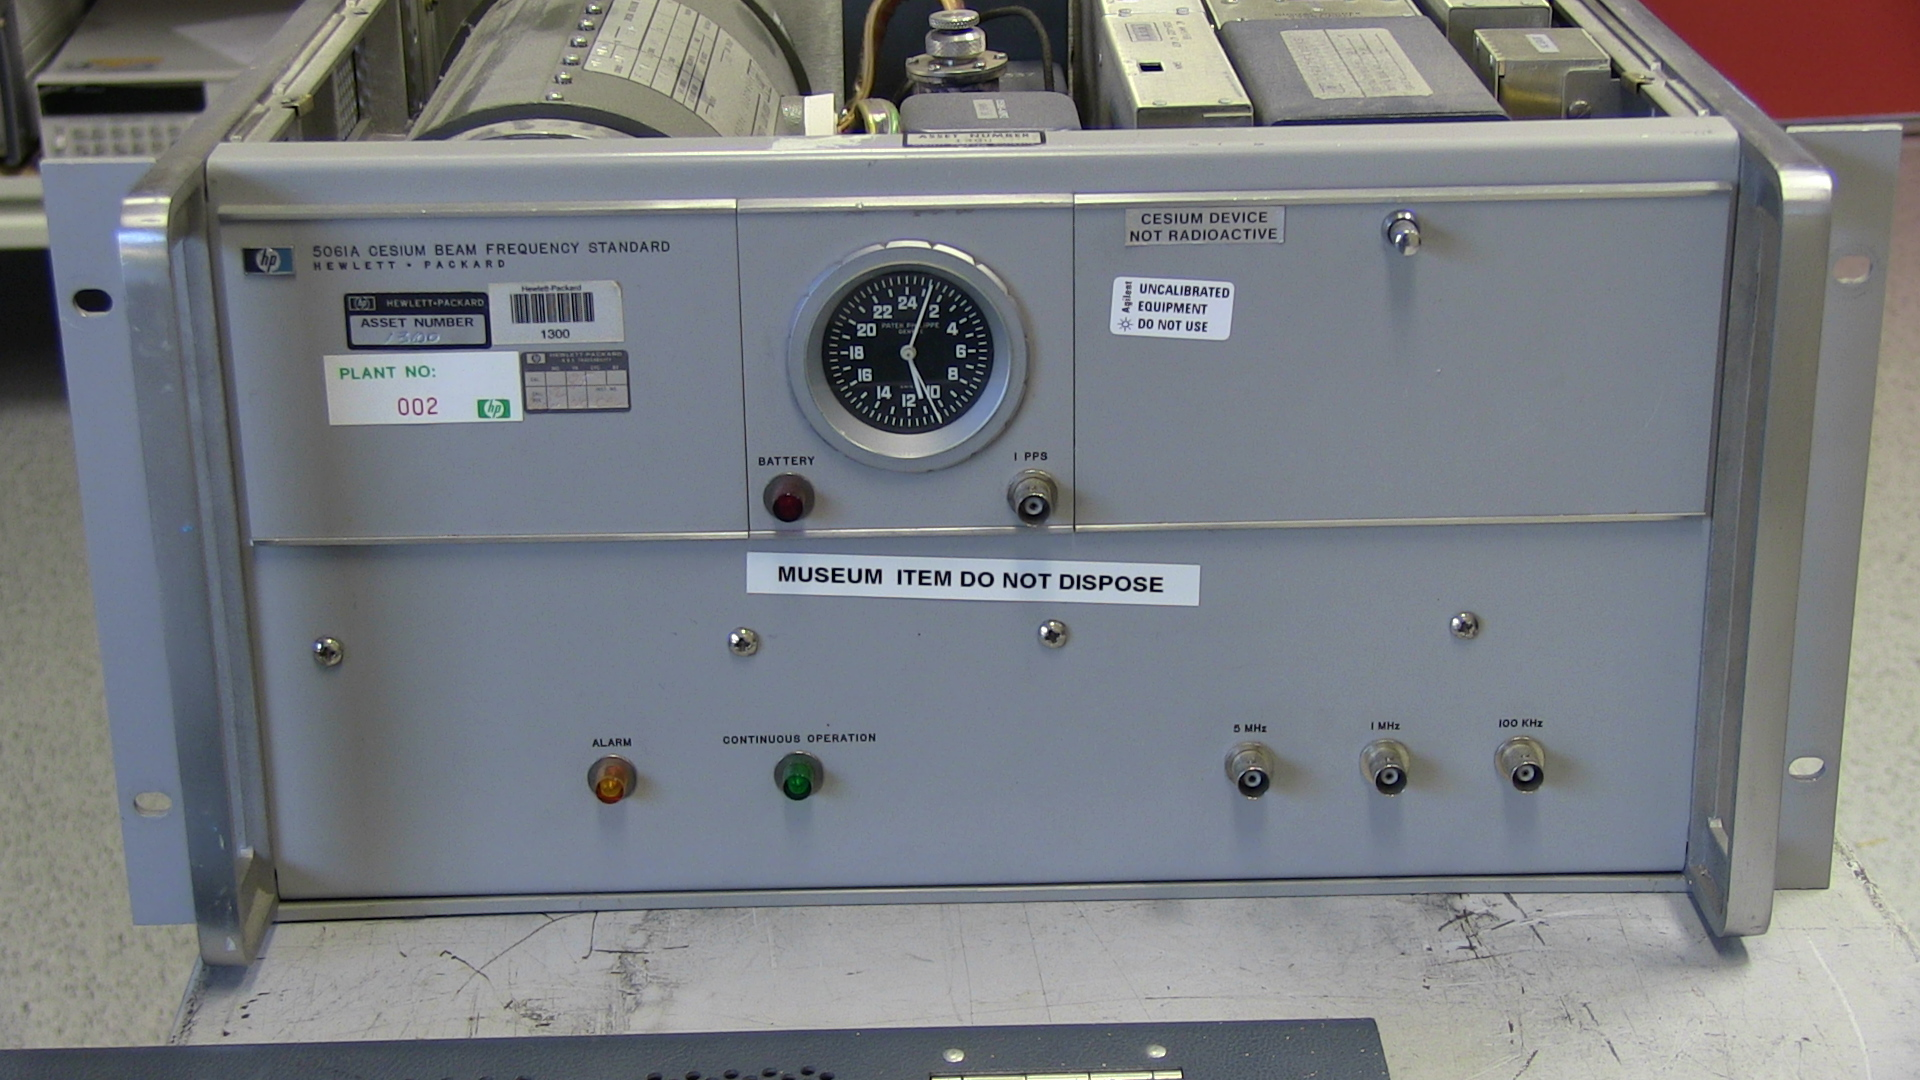
\includegraphics[width=\textwidth]{fig/atomicClock.JPG}\\
                        {\tiny Picture by Dave L. Jones}
      }
      
      \only<2>{
        ~
        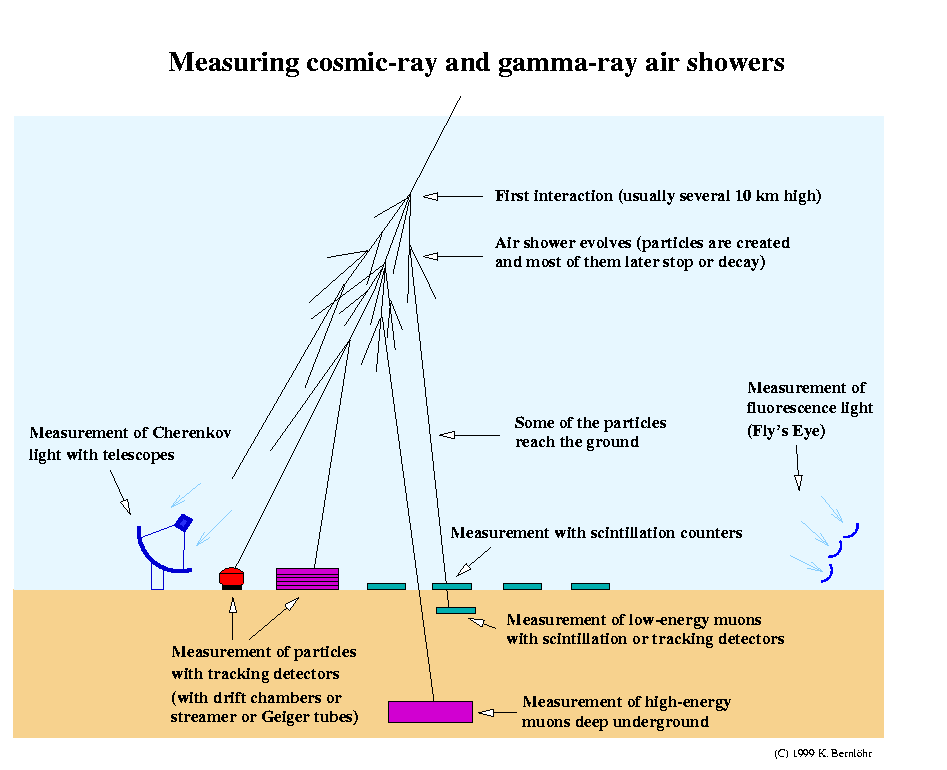
\includegraphics[width=\textwidth]{fig/muon.png}\\
                        {\tiny Figure by K.Bernkör}
      }
      
      \only<3>{
        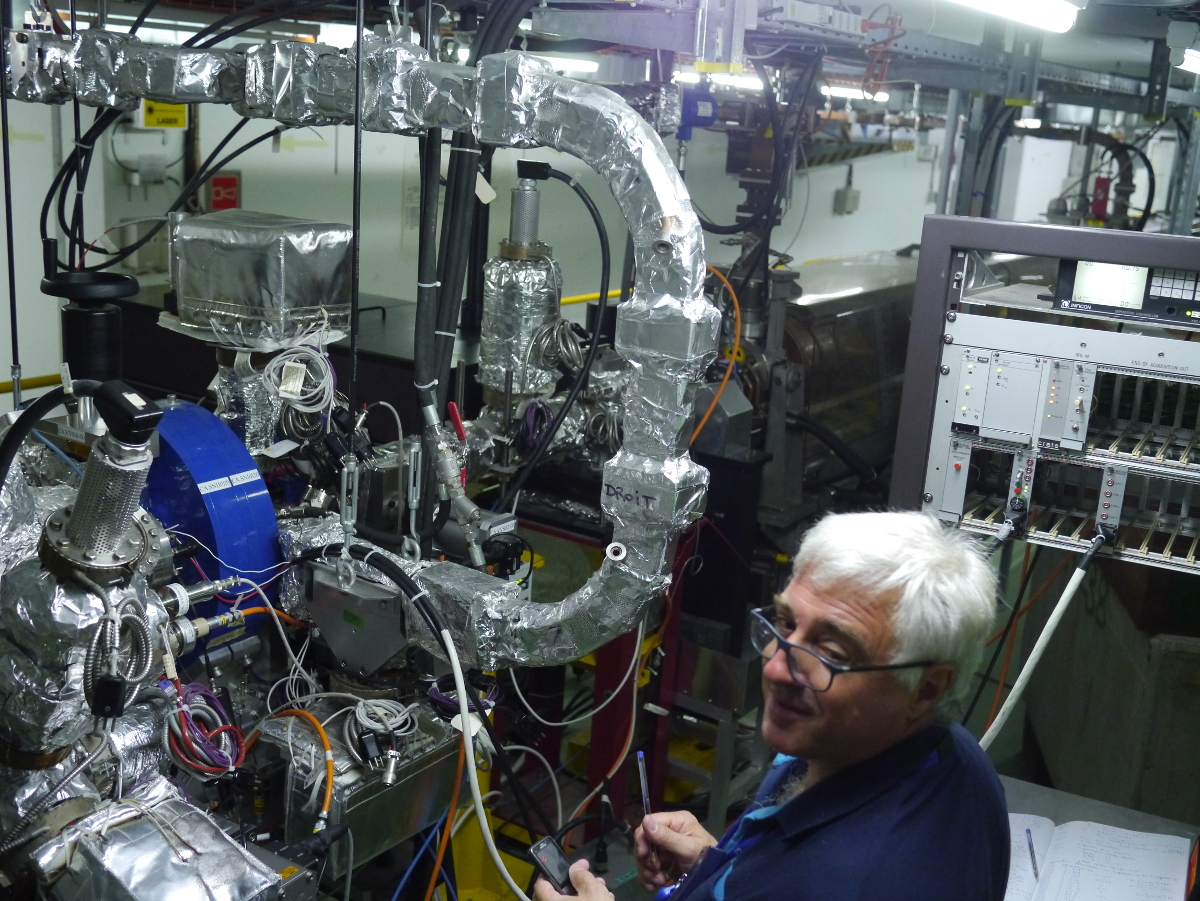
\includegraphics[width=\textwidth]{fig/Clear_Scale.JPG}\\
                        {\tiny Photo by K.Sjøbæk}
      }
      
      %%   %Without time delation, the particles themselves experience the time to be shorter from one end of the accelerator to the other or that we see them as taking longer time. Therefore the bunch of electrons, as you see here in CLEAR would blow up much more and not be useful in the end
      %%   \end{itemize}
      
    \end{column}
  \end{columns}
\end{frame}

\section{General relativity}

\begin{frame}{Is gravity acceleration}
  \begin{columns}
    \begin{column}{0.5\textwidth}
      \begin{itemize}
      \item{In 1907 Einstein had the ``happiest thought of his life''}
      \item<2->{There is no difference between being in an accelerated elevator in space or being in a gravitational field}
      \item<4->{This was a continuation of the the universality of free fall}
         
        %% \item{Two masses fall with the same accelration already seen by Galelio}
      %% \item{This lead Einstin to think: What if accelration is the same as gravity, would we know the difference}
      %% \item{Locally space can be though about as a free falling cordinate system}
      %%   \item{Free fall is where no forces is acting}
      %%   \item{We only feel gravity because the earth is massiv, so we resist the free fall}
      %% \item{Yes, you would if you where 30000 m long}
      %% \item{What if gravity was only a result of a geometry}
        \end{itemize}
         \end{column}

    \begin{column}{0.5\textwidth}
      %\begin{center}
        \begin{tikzpicture}
         % \node at (1,-4) {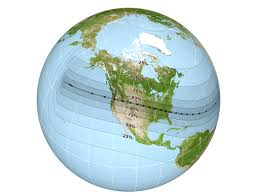
\includegraphics[width=1\textwidth]{fig/theEarth.jpg}};

        \def\x{2}
        \def\h{4}
        \def\xn{0}
        \def\hn{0}
        
        \only<2>{
          \node at (1,1.2) {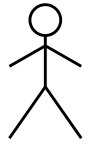
\includegraphics[width=0.25\textwidth]{fig/streken.png}};
          \path[lineP,green, line width=0.3cm] (-1,\hn-0.12cm)--(3,\hn-0.12cm);
          \node at (1,1.2) {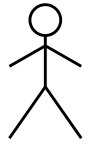
\includegraphics[width=0.25\textwidth]{fig/streken.png}};
        \path[lineP] (\hn,\xn)--(\xn,\h);
        \path[lineP] (\xn,\h)--(\x,\h);
        \path[lineP] (\x,\h)--(\x,\hn);
        \path[lineP] (\xn,\hn)--(\x,\hn);
        %\path[lineP,green] (-1,\hn)--(3,\hn);
        \node at (2.5,0.4) {
\includegraphics[width=0.07\textwidth]{fig/flower.png}};
         \node at (-0.5,0.4) {
\includegraphics[width=0.17\textwidth]{fig/grass.png}};
              }
        %% \def\x{4}
        %% \def\h{2}
        %% \def\xn{3}
        %% \def\hn{0}
        \only<3,4>{
        \draw [draw=black,fill=blue!30!black] (-1,-1) rectangle (4,5);
        \draw [draw=black,fill=white] (\xn,\hn) rectangle (\x,\h);  
        \path[lineP] (\xn,\hn)--(\xn,\h);
        \path[lineP] (\xn,\h)--(\x,\h);
        \path[lineP] (\x,\h)--(\x,\hn);
        \path[lineP] (\xn,\hn)--(\x,\hn);
        \node[star, star points=5, minimum width=0.1cm,inner sep=1.8pt,anchor=outer point 3,star point ratio=5.25, fill=yellow, draw] at (3,0.5) {};
        \node[star, star points=5, minimum width=0.1cm,inner sep=1.8pt,anchor=outer point 3,star point ratio=5.25, fill=yellow, draw] at (2.2,1.5) {};
        \node[star, star points=5, minimum width=0.1cm,inner sep=1.8pt,anchor=outer point 3,star point ratio=5.25, fill=yellow, draw] at (-0.8,1.0) {};
        \node[star, star points=5, minimum width=0.1cm,inner sep=1.8pt,anchor=outer point 3,star point ratio=5.25, fill=yellow, draw] at (0,4.2) {};
        \node[star, star points=5, minimum width=0.1cm,inner sep=1.8pt,anchor=outer point 3,star point ratio=5.25, fill=yellow, draw] at (2.5,3.7) {};
        \node at (1,1.2) {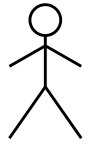
\includegraphics[width=0.25\textwidth]{fig/streken.png}};



 \filldraw[fill=yellow!70!red, draw=yellow!10!red] (0.5,0)--(0.6,-0.5)--(0.7,-0.1)--(0.8,-0.8)--(0.9,-0.1)--(1.0,-1.0)--(1.1,-0.1)--(1.2,-0.8)--(1.3,-0.1)--(1.4,-0.5)--(1.5,0);


        }
        %\draw[ultra thick] (1,2.3) circle (0.3cm);
        %\path[lineP] (0.3,1.4)--(1.0,1.8);
        %\path[lineP] (1.7,1.4)--(1.0,1.8);
        %\draw[ultra thick] (1,2.3) circle (0.3cm);
   \end{tikzpicture}
%\end{center}
    \end{column}
  \end{columns}
\end{frame}


\begin{frame}{Is gravity a geometrical effect}
  \begin{columns}
    \begin{column}{0.4\textwidth}
      \begin{itemize}
      \item<1->{The equivalence principle is only valid locally}
      \item<2->{Globally there is tidal forces}
      \item<4->{Can gravity be a geometrical effect}
      \end{itemize}
    \end{column}
    \begin{column}{0.6\textwidth}
      \begin{center}
      \begin{tikzpicture}

        
        \def\x{2}
        \def\h{3}
        \def\xn{-2}
        \def\hn{1}
        
        %% \path[lineP] (\xn,\hn)--(\xn,\h);
        %% \path[lineP] (\xn,\h)--(\x,\h);
        %% \path[lineP] (\x,\h)--(\x,\hn);
        %% \path[lineP] (\xn,\hn)--(\x,\hn);

        \only<2>{
        \node[circle,ball color=red,shading=ball,minimum width=3cm] (ball1) at (0,-2) {};

        \node[circle,ball color=black,shading=ball,minimum width=0.3cm] (ball2) at (1,2.5) {};

        \node[circle,ball color=black,shading=ball,minimum width=0.3cm] (ball3) at (-1,2.5){};

        \path[lineP,gray,dotted] (ball1)--(ball2);
        \path[lineP,gray,dotted] (ball1)--(ball3);
        }


        \only<3,4>{
        \def\R{3 } % sphere radius
        \def\angEl{20} % elevation angle
        \def\angAz{-20} % azimuth angle
        \filldraw[shading=ball,ball color=blue] (0,0) circle (\R);
        %\filldraw[fill=white] (0,0) circle (\R);
        
        \foreach \t in {0} { \DrawLatitudeCircle[\R]{\t} }
        \foreach \t in {0,30,60,90,120,150} { \DrawLongitudeCircle[\R]{\t} }
        }
        \only<3>{
        \node[circle,ball color=black,shading=ball,minimum width=0.3cm] (ball2) at (1.5,-0.9) {};
        
        \node[circle,ball color=black,shading=ball,minimum width=0.3cm] (ball3) at (-1.5,-0.9){};
        }
        
        \only<4>{
        \node[circle,ball color=black,shading=ball,minimum width=0.3cm] (ball2) at (0.8,1.9) {};
        
        \node[circle,ball color=black,shading=ball,minimum width=0.3cm] (ball3) at (-0.8,1.9){};
        }
        
      \end{tikzpicture}
      \end{center}
    \end{column}
  \end{columns}
\end{frame}



\begin{frame}{A geometrical model for gravity}
\begin{itemize}
\item{General relativity describes spacetime as a manifold}
\item{A manifold can describe a space that locally is flat, but is curved on larger scale}
\uncover<2->{
\item{The surface of a sphere:}
  \begin{itemize}
  \item{Curved on larger scale}
  \item{Locally flat}
  \end{itemize}
}
\uncover<3->{
\item{Spacetime according to general relativity}
  \begin{itemize}
  \item{Locally it a free falling coordinate system, the weak equivalence principle holds}
  \item{Curved spacetime on larger scale}
  \end{itemize}
  }
\item<4->{Describing spacetime as a manifold gave the theory a  mathematical framework (tensor analysis)}
\end{itemize}
\end{frame}
  
\begin{frame}{Einsteins field equations}
  \begin{columns}
    \begin{column}{0.5\textwidth}
      \begin{itemize}
      %% %\item{By describing space by this manifold, and requireing that Newtons mechanics holds for low energies the Einstein field equation was derived}
      %% \item{Left side describes the curvature of space, only depends on the metric $g_{\mu_nu}$}
      %% \item{The metric is the input to the geodesic equation}%, that gives the paths objects will move if no force is acting}
      %% \item{$\Lambda$ is the cosmological constant}
      %% \item{$T_{\mu \nu}$ is the stress-energy tensor, and describes the density and flux of energy in spacetime}
      %% \item{Only solvable in special cases, for instance the Schwarzshild solution}

           %\item{By describing space by this manifold, and requireing that Newtons mechanics holds for low energies the Einstein field equation was derived}
      \item<1->{Left side describes the curvature of space}
      \item<1->{Right side describes the content of space}
      \item<2->{The metric,$g_{\mu_\nu}$, is what we want to solve for} 
      \item<3->{The metric is the input to the geodesic equation}%, that gives the paths objects will move if no force is acting}
      \item<4->{Only solvable in special cases, for instance the Schwarzshild solution}
      \end{itemize}
    \end{column}
    \begin{column}{0.6\textwidth}
      \centering
      \footnotesize
      Field equations
      \tiny
  \begin{empheq}[box=\tcbhighmath]{align*}
    R_{\mu \nu} - {1 \over 2}g_{\mu \nu}\,R + g_{\mu \nu} \Lambda &= 
    {8 \pi G \over c^4} T_{\mu \nu}
   % R=\text{Ricci curvature tensor} (f(g_{\mu_\nu})
  \end{empheq}
  \begin{empheq}[box=\tcbhighmath]{align*}
    R_{\mu_\nu}&=\text{Ricci curvature tensor} (f(g_{\mu_\nu}))\\
    g_{\mu_\nu}&=\text{The metric}\\
    \Lambda&=\text{Cosmological constant}\\
    T_{\mu \nu}&=\text{Stress-energy tensor}
  \end{empheq}
  \footnotesize
 \visible<3->{
  The geodesic equation
  \tiny
      \begin{empheq}[box=\tcbhighmath]{align*}
        \frac{d^2x^{\mu}}{ds^2}+
        \Gamma^{\mu}_{\hphantom{\mu}\beta\alpha} \frac{d^2x^{\alpha}}{ds^2} \frac{d^2x^{\beta}}{ds^2}=0\\
        \Gamma^{\mu}_{\hphantom{\mu}\beta\alpha}=\text{Christoffel sybol}(f(g_{\mu_\nu}))
      \end{empheq}
      }
  \end{column}
  \end{columns}
\end{frame}




\begin{frame}{Gravitational redshift}
  \begin{center}
    \begin{tikzpicture}
      \def\x{4}
      \def\h{6}
      \def\xn{-1}
      \def\hn{0}
      \only<1->{
        \draw [draw=black,fill=blue!30!black] (-4,-1) rectangle (7,7);
        \draw [draw=black,fill=white] (\xn,\hn) rectangle (\x,\h);  
        \path[lineP] (\xn,\hn)--(\xn,\h);
        \path[lineP] (\xn,\h)--(\x,\h);
        \path[lineP] (\x,\h)--(\x,\hn);
        \path[lineP] (\xn,\hn)--(\x,\hn);
        %\node[star, star points=5, minimum width=0.1cm,inner sep=1.8pt,anchor=outer point 3,star point ratio=5.25, fill=yellow, draw] at (3,0.5) {};
        \node[star, star points=5, minimum width=0.1cm,inner sep=1.8pt,anchor=outer point 3,star point ratio=5.25, fill=yellow, draw] at (5.2,1.5) {};
        \node[star, star points=5, minimum width=0.1cm,inner sep=1.8pt,anchor=outer point 3,star point ratio=5.25, fill=yellow, draw] at (-2.8,2.0) {};
      \node[star, star points=5, minimum width=0.1cm,inner sep=1.8pt,anchor=outer point 3,star point ratio=5.25, fill=yellow, draw] at (0,6.0) {};
      %\node[star, star points=5, minimum width=0.1cm,inner sep=1.8pt,anchor=outer point 3,star point ratio=5.25, fill=yellow, draw] at (2.5,3.7) {};
    }
    %\only<1>{
    %  \node at (2,2.2) {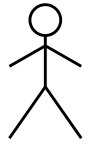
\includegraphics[width=0.10\textwidth]{fig/streken.png}};
    %}
      \only<2>{
        \path[draw](-1,3)--(0.1,3);
        \path[draw](-1,3.5)--(1.9,3.5);
        \draw [decorate,decoration={brace,amplitude=10pt},rotate=0]
        (0.0,3) -- (0.0,0) node [xshift=0.5cm,yshift=1.5cm] {\tiny y};
        \path[light](0.0,0)--(0.0,3);
        \draw [decorate,decoration={brace,amplitude=10pt},rotate=0]
        (1.8,3.5) -- (1.8,0) node [xshift=0.7cm,yshift=1.4cm] {\tiny y$+\lambda$};
        \path[light](1.8,0)--(1.8,3.5);
        \draw [decorate,decoration={brace,amplitude=2pt},rotate=0]
        (-0.8,3.5) -- (-0.8,3) node [xshift=0.3cm,yshift=0.2cm] {\tiny $\lambda$};
      }
      
      \only<3->{
        \path[draw](-1,3.1)--(0.1,3.1);
         \path[draw](-1,3.7)--(1.9,3.7);
     \draw [decorate,decoration={brace,amplitude=10pt},rotate=0]
      (0.0,3.1) -- (0.0,0) node [xshift=0.85cm,yshift=1.55cm] {\tiny y+$\frac{1}{2}a\frac{y^2}{c^2}$};
      \path[light](0.0,0)--(0.0,3.1);
      \draw [decorate,decoration={brace,amplitude=10pt},rotate=0]
      (1.8,3.7) -- (1.8,0) node [xshift=1.15cm,yshift=1.45cm] {\tiny y$+\lambda\frac{1}{2}a\frac{(y+\lambda)^2}{c^2}$};
      \path[light](1.8,0)--(1.8,3.7);
      \draw [decorate,decoration={brace,amplitude=2pt},rotate=0]
      (-0.8,3.7) -- (-0.8,3.1) node [xshift=0.55cm,yshift=0.3cm] {\tiny $\lambda+\frac{gy\lambda}{c²}$};

      \filldraw[fill=yellow!70!red, draw=yellow!10!red,xshift=-0.3cm,scale=2] (0.5,0)--(0.6,-0.5)--(0.7,-0.1)--(0.8,-0.8)--(0.9,-0.1)--(1.0,-1.0)--(1.1,-0.1)--(1.2,-0.8)--(1.3,-0.1)--(1.4,-0.5)--(1.5,0);
      }
      \only<4->\node at (1,4.0) {\footnotesize Redshift depends upon y};
    \end{tikzpicture}
    \end{center}
\end{frame}











%% \begin{frame}{Gravitational redshift}
%%   \begin{columns}
%%     \begin{column}{0.5\textwidth}
%%       \begin{itemize}
%%       %\item{Gravitational redshift can be understood just by the equivalence principle}
%%       %\item{Hight above the floor when the elevator is free falling is y}
%%       %\item{Now a light is emmitted from the bottom of the elevator}
%%       %\item{If the elevator is accelerated the path the light has to travel becomes:$y'(y)=y+\frac{g}{2}\left(\frac{y}{c}\right)...$}
%%       \item{Line segment $\lambda$}
%%       \item{$y'(y+\lambda)=y+\lambda+\frac{g}{2}\left(\frac{y+\lambda}{c}\right)-y+\frac{g}{2}\left(\frac{y}{c}\right)=\lambda+\frac{gy\lambda}{c²}+\frac{1g\lambda^2}{2c^2}\approx \lambda+\frac{gy\lambda}{c²}$}

%%       \item{As seen the the wavelength increases as a function of y, this is the gravitational redshift}
%%       \item{The frequency of the lights can not be changed, because then the light would be fill up the elevator, more lightwaves in than out}
%%       \item{In order to get all the waves out of the elevator the time also has to move faster at the top of the elevator}
%%       \item{Gravitational time dilation, important for GPS clocs}
        
%%       %% \item{What happens to a length interval $\lambda$ in a gravitational field}
%%       %% \item{Lets first assume the elevator is in free fall, then define the hight of the elevator at any point as y}
%%       %% \item{A light beam travels from the bottom of the elevator to the point y}
%%       %% \item{Let see how far the light has to travel to get to the same point y in the accelerated frame of reference}
%%       %% \item{Now lets see what happens with an }
%%       \end{itemize}
%%     \end{column}
%%     \begin{column}{0.5\textwidth}
%%       \begin{tikzpicture}
%%         \def\x{2}
%%         \def\h{4}
%%         \def\xn{0}
%%         \def\hn{0}
%%         \only<1->{
%%         \draw [draw=black,fill=blue!30!black] (-1,-1) rectangle (4,5);
%%         \draw [draw=black,fill=white] (\xn,\hn) rectangle (\x,\h);  
%%         \path[lineP] (\xn,\hn)--(\xn,\h);
%%         \path[lineP] (\xn,\h)--(\x,\h);
%%          \path[lineP] (\x,\h)--(\x,\hn);
%%          \path[lineP] (\xn,\hn)--(\x,\hn);
%%          \node[star, star points=5, minimum width=0.1cm,inner sep=1.8pt,anchor=outer point 3,star point ratio=5.25, fill=yellow, draw] at (3,0.5) {};
%%          \node[star, star points=5, minimum width=0.1cm,inner sep=1.8pt,anchor=outer point 3,star point ratio=5.25, fill=yellow, draw] at (2.2,1.5) {};
%%          \node[star, star points=5, minimum width=0.1cm,inner sep=1.8pt,anchor=outer point 3,star point ratio=5.25, fill=yellow, draw] at (-0.8,1.0) {};
%%          \node[star, star points=5, minimum width=0.1cm,inner sep=1.8pt,anchor=outer point 3,star point ratio=5.25, fill=yellow, draw] at (0,4.2) {};
%%          \node[star, star points=5, minimum width=0.1cm,inner sep=1.8pt,anchor=outer point 3,star point ratio=5.25, fill=yellow, draw] at (2.5,3.7) {};
%%         }
%%         \only<1>{
%%          \node at (1,2.2) {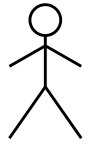
\includegraphics[width=0.25\textwidth]{fig/streken.png}};
%% }
         
%%         \only<2->{
%%            \draw [decorate,decoration={brace,amplitude=10pt},rotate=0]
%%            (1.0,3) -- (1.0,0) node [xshift=0.5cm,yshift=1.5cm] {\textbf{y}};
%%         }
        
%%         \only<3>{
%%           \path[light](1.0,0)--(1.0,3);
       
%%          }
%%         \end{tikzpicture}
%%     \end{column}
%%   \end{columns}
%% \end{frame}


%% \begin{frame}{Gravity and frequency of light and your GPS}
%%   \begin{columns}
%%     \begin{column}{0.5\textwidth}
%%       \begin{itemize}
%%       \item{Given that the equivalence principle holds, what happens with light  emitted from the floor}
%%       \end{itemize}
%%     \end{column}
%%     \begin{column}{0.5\textwidth}
%%       \includegrapics{fig/solar.jpg}
%%     \end{column}
%%   \end{columns}
%% \end{frame}
  

\begin{frame}{Gravity and light}
  \begin{columns}
    \begin{column}{0.5\textwidth}
     \begin{itemize}
       \item{Light is being bent by gravitational fields}
       %\item{What happens to position of stars}
       %\item{This can be tested, when there is a solar eclipse}
       \end{itemize}
    \end{column}
    \begin{column}{0.5\textwidth}


 \begin{tikzpicture}
        \def\x{2}
        \def\h{4}
        \def\xn{0}
        \def\hn{0}
        \only<1,2>{
        \draw [draw=black,fill=blue!30!black] (-1,-1) rectangle (4,5);
        \draw [draw=black,fill=white] (\xn,\hn) rectangle (\x,\h);  
        \path[lineP] (\xn,\hn)--(\xn,\h);
        \path[lineP] (\xn,\h)--(\x,\h);
         \path[lineP] (\x,\h)--(\x,\hn);
         \path[lineP] (\xn,\hn)--(\x,\hn);
         \node[star, star points=5, minimum width=0.1cm,inner sep=1.8pt,anchor=outer point 3,star point ratio=5.25, fill=yellow, draw] at (3,0.5) {};
         \node[star, star points=5, minimum width=0.1cm,inner sep=1.8pt,anchor=outer point 3,star point ratio=5.25, fill=yellow, draw] at (2.2,1.5) {};
         \node[star, star points=5, minimum width=0.1cm,inner sep=1.8pt,anchor=outer point 3,star point ratio=5.25, fill=yellow, draw] at (-0.8,1.0) {};
         \node[star, star points=5, minimum width=0.1cm,inner sep=1.8pt,anchor=outer point 3,star point ratio=5.25, fill=yellow, draw] at (0,4.2) {};
         \node[star, star points=5, minimum width=0.1cm,inner sep=1.8pt,anchor=outer point 3,star point ratio=5.25, fill=yellow, draw] at (2.5,3.7) {};
        
       
         \node at (0.5,0.65) {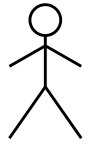
\includegraphics[width=0.15\textwidth]{fig/streken.png}};
         }
        \only<1>{\draw[ultra thick,yellow] (0.75,0.75) parabola (1.8,0.75);}
        \only<2>{\draw[ultra thick,yellow] (0.75,0.75) parabola (1.8,0.4);
        %\filldraw[fill=blue, draw=yellow, line width=3mm] (0, 0)-- (2, 1)--(0,2)--(1,1) circle;
          \filldraw[fill=yellow!70!red, draw=yellow!10!red] (0.5,0)--(0.6,-0.5)--(0.7,-0.1)--(0.8,-0.8)--(0.9,-0.1)--(1.0,-1.0)--(1.1,-0.1)--(1.2,-0.8)--(1.3,-0.1)--(1.4,-0.5)--(1.5,0);
          }
 \end{tikzpicture}
      %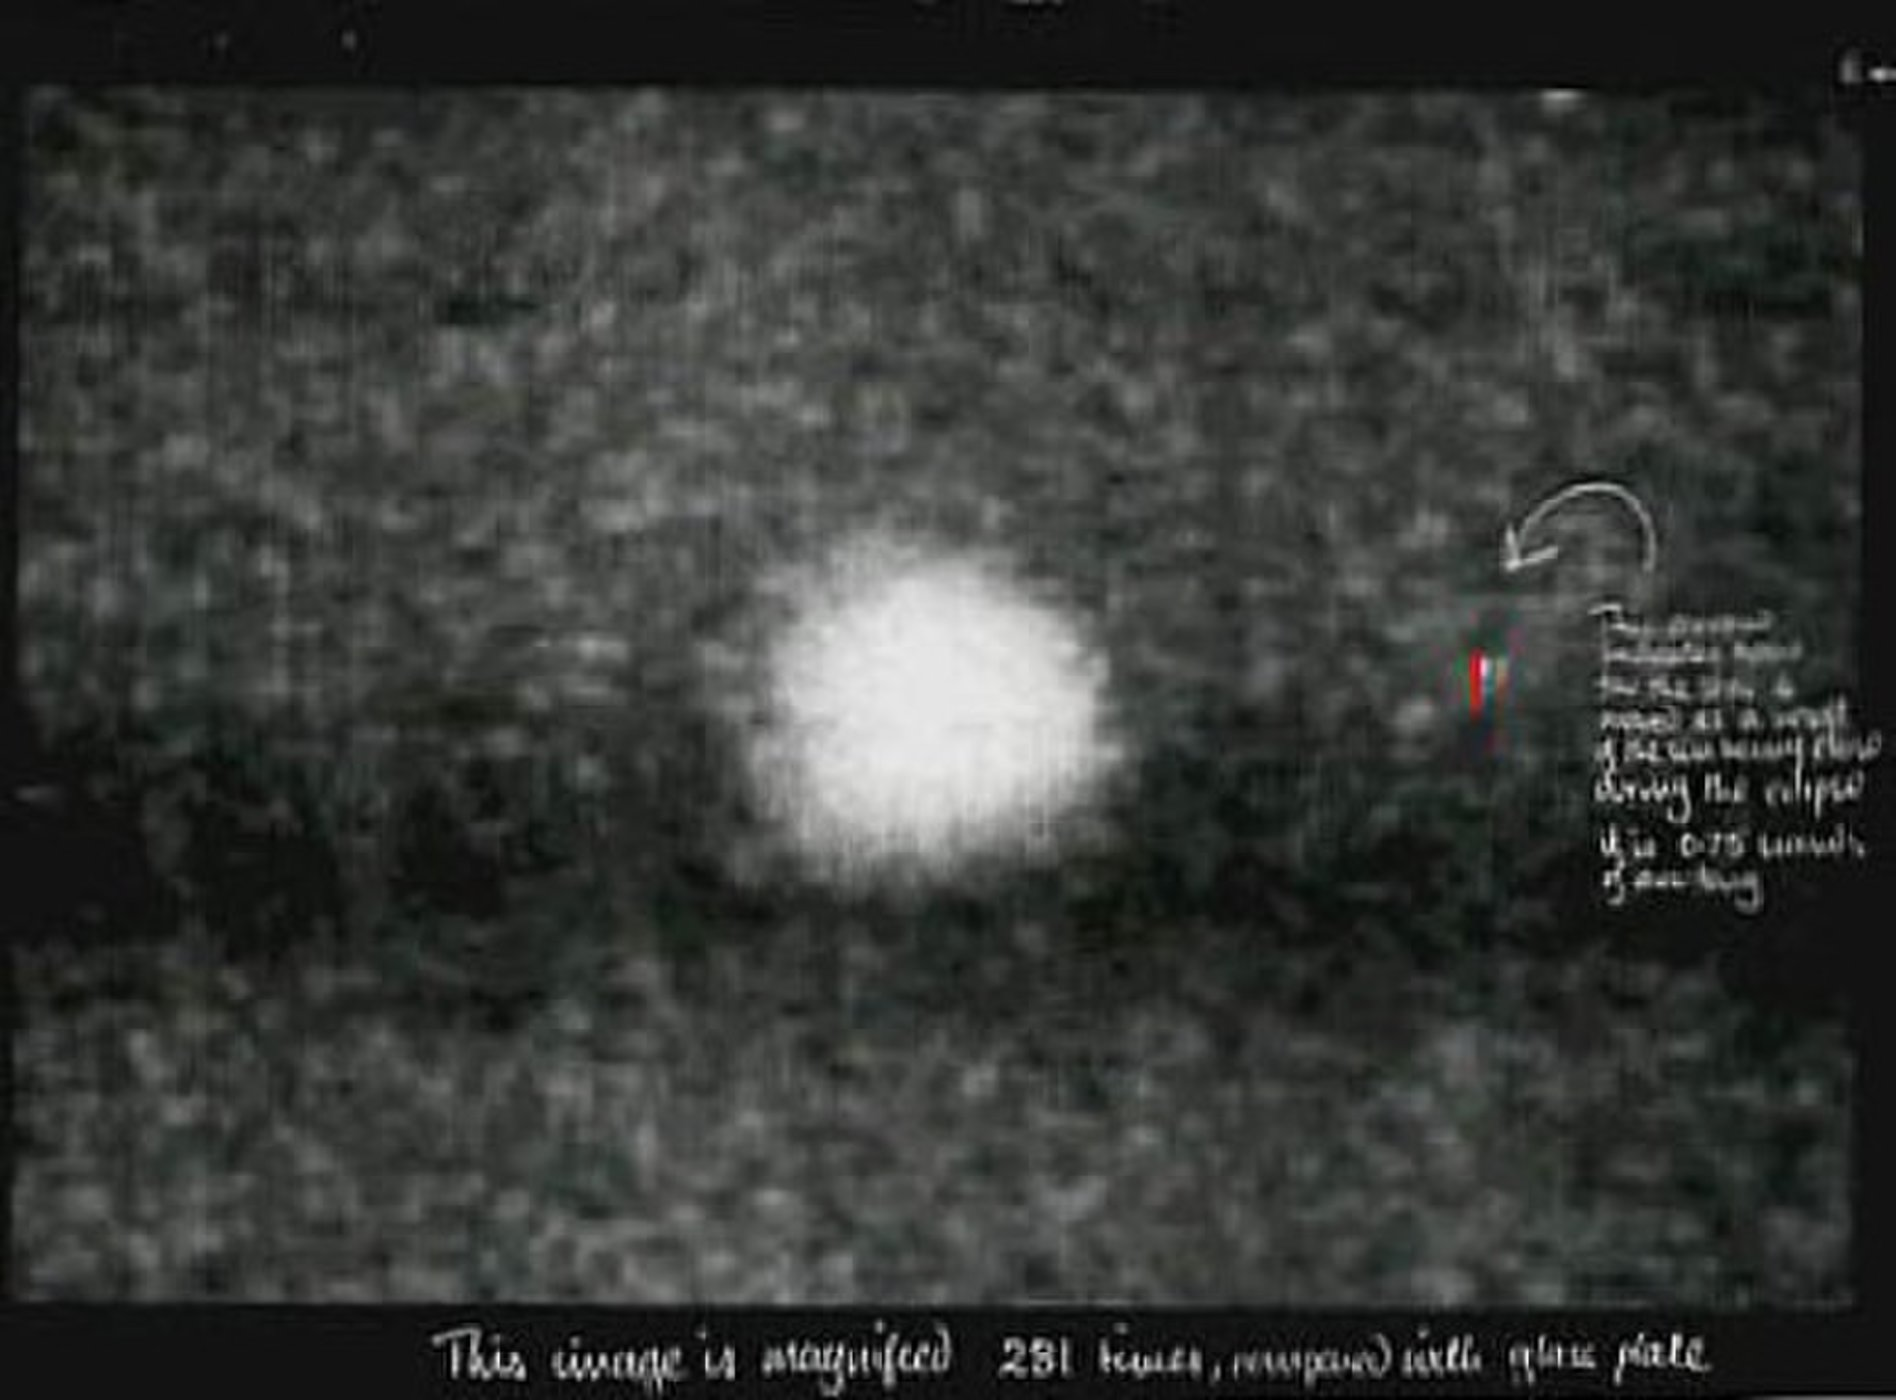
\includegraphics{fig/solar.jpg}
    \end{column}
 \end{columns}
 \end{frame}
  
\begin{frame}{Testing the theory}
  %\begin{columns}
  %  \begin{column}{0.5\textwidth}
     \begin{itemize}
       \item<1->{Bending of light by the sun might alter the position of stars}
       %\item{Only possible to see during a solor eclipse}
       \item{Solar eclipse 1919 was the ultimate test}
    %   \end{itemize}
         %  \end{column}
         %  \begin{column}{0.5\textwidth}
         % \begin{itemize}
         \item{Three possible outcome}
         \begin{itemize}
         \item{No bending}
         \item{Newton bending}
         \item{Bending of light predicted by General relativity}
         \end{itemize}
       \item{Turned out that GR was right}
    \end{itemize}
  %  \end{column}
  %  \end{columns}

  \begin{tikzpicture}
    \node[star, star points=5, minimum width=0.1cm,inner sep=1.0pt,anchor=outer point 3,star point ratio=3.25, fill=gray, draw] at (-1,3) {};
    \draw [yellow] plot [smooth] coordinates {(0,0) (2,0.1) (4,1.1) (6,0.8) (10,0)};
    \draw [yellow] (0,0) --(10,0);
    %\draw [yellow] plot [smooth] coordinates {(0,0) (2,0.8) (4,1.1) (6,0.8) (10,0)};
    \node at (5,0){
\includegraphics[width=1cm]{fig/sun.png}};
  \end{tikzpicture}

 \end{frame}




\end{document}
%% \path[lineP] (0.3,0)--(1,1);
%% \path[lineP] (1,1)--(1.7,0);
%% \path[lineP] (1,1)--(1,2);
%% \path[lineP] (0.3,1.4)--(1.0,1.8);
%% \path[lineP] (1.7,1.4)--(1.0,1.8);
%% \draw[ultra thick] (1,2.3) circle (0.3cm);
        
        
